\documentclass[10pt,journal,compsoc,twoside]{IEEEtran}


\ifCLASSINFOpdf
  \usepackage[pdftex]{graphicx}
  \graphicspath{{./figures/}}
  \DeclareGraphicsExtensions{.pdf,.jpeg,.png}
\fi
\usepackage{amsmath}
\usepackage{amssymb}
\usepackage{amsmath}
\usepackage{amsfonts}
\usepackage{mathtools}
\usepackage[utf8]{inputenc}
\usepackage{csquotes}
\usepackage[english]{babel}
\usepackage[T1]{fontenc}
\usepackage{color}
\usepackage{nth}
\usepackage{hyperref}
\usepackage{nameref}

\usepackage{graphicx}

\hypersetup{
     colorlinks   = true,
     citecolor    = blue,
     filecolor=cyan,      
     urlcolor=magenta,
}
\usepackage{cleveref}
\usepackage{listings}
\definecolor{codegreen}{rgb}{0,0.4,0}
\lstset{
    frameround=fttt,
    language=python,
    numbers=left,
    breaklines=true,
    keywordstyle=\color{blue}\bfseries, 
    basicstyle=\ttfamily\color{black},
    numberstyle=\color{black},
    stringstyle=\color{codegreen},
    }
\lstdefinelanguage{none}{
  identifierstyle=
}
\hyphenation{op-tical net-works semi-conduc-tor}
\newcommand{\matr}[1]{\mathbf{#1}} % undergraduate algebra version
\renewcommand{\vec}[1]{\mathbf{#1}} %if bold vectors wanted
\DeclareMathOperator*{\argmin}{arg\,min}
\DeclareMathOperator*{\argmax}{arg\,max}

\begin{document}
\suppressfloats
\title{Assignment 5 \\ GridWorld}
\author{Jonas Kulhanek}
\markboth{LS2018, Assignment 5 --- GridWorld}%
{B4B36ZUI, BE4B36ZUI}
\IEEEtitleabstractindextext{%
\begin{abstract}

    %TODO:
This paper is the result of my assignment concerned with dynamic programming.
In the assigment I worked with python to implement some algorithms used in dynamic programming
and did some tests on them.
\end{abstract}
}
\maketitle
\section{Introduction}\label{sec:introduction}
\IEEEPARstart{T}{he} objective of this assignment was to experiment with reinforcement learning techniques. Specifically with dynamic programming.
In the implementation part, I was supposed to implement value iteration and policy iteration techniques used in dynamic programming.
In the experiment part I work with them to get some insight and to learn effectively, how they work.
The experiments presented here are implemented in python jupyter notebooks. They are included in the homework.
In the source code I used python with numpy library.


\section*{Experiment 1}\label{sec:experiment1}
\begin{figure}
    \caption{Plot showing how values of selected states of game 3x4 changes with change in probability.}
    \label{fig:experiment1}
    \centering
        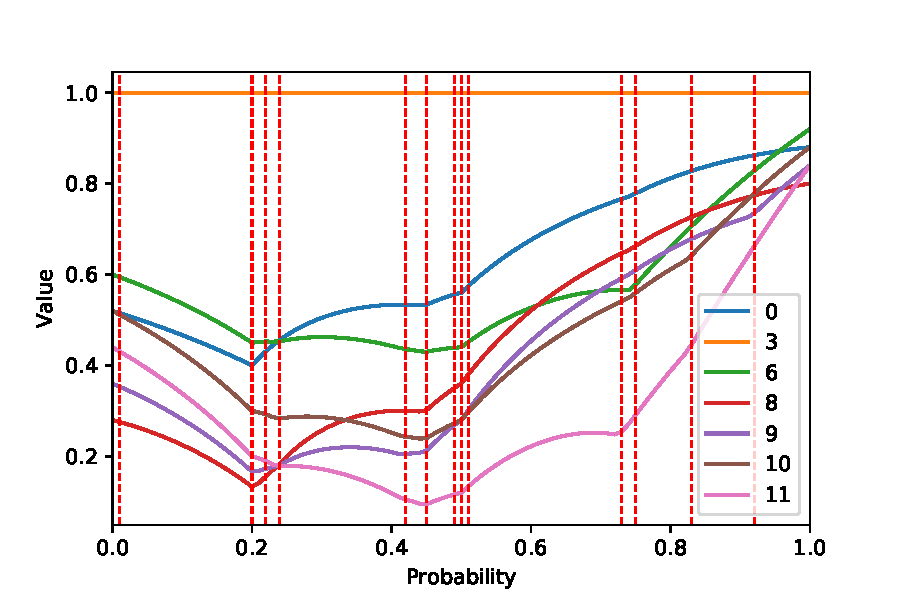
\includegraphics[width=0.5\textwidth, angle=0]{figures/e1.pdf}
\end{figure}
In this experiment I analyzed how the valuation of selected
states changed with a change in probability. The experiment was
analyzed on the 3x4 board. I calculated the value for probabilities taken
uniformly from the interval [0,1]. The result can be seen in
figure \ref{fig:experiment1}. A vertical line represents the probability,
where a policy change occurs. Furthermore, those probabilities are given in the following table.
\begin{center}
    \begin{tabular}{ | c | c | c | c | c |  c| c |}
      \hline
      0.01 & 0.2 & 0.22 & 0.24 & 0.42 & 0.45 & 0.49 \\ \hline
       0.5 & 0.51 & 0.73 & 0.75 & 0.83 & 0.92 & \\
      \hline
    \end{tabular}
  \end{center}

It can be seen, that on the places, where the policy was changed, the value of the board started increasing again.

\section*{Experiment 2}\label{sec:experiment2}


In the second experiment, I analyzed, how the policy changed with a change in transition cost.
The experiment was done on 5x5 board.
Because, I needed to test it on unbounded interval - [0, $\infty$),
I took the [0, 1) interval and transformed it using a function, that stretched it to the desired interval.
For the details on the used function, please refer to \nameref{sec:transform_function}
The change in policy occured on those values:


\begin{center}
    \begin{tabular}{ | c | c | c | c | c |  c| c |}
        \hline
        0.02 & 0.27 & 0.34 & 0.38 & 0.46 & 0.64 & 0.96 \\ \hline
         1.04 & 2.00 & 2.92 & 3.24 & & & \\ \hline
    \end{tabular}
\end{center}

The 5x5 board can be seen in the figure \ref{fig:e2board}

\begin{figure}
    \caption{The 5x5 board}
    \label{fig:e2board}
        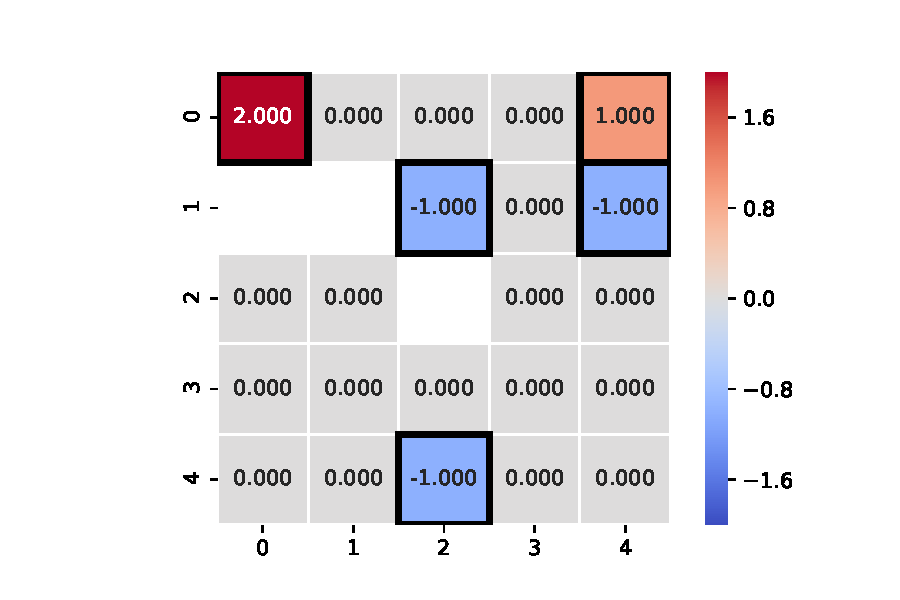
\includegraphics[width=0.5\textwidth, angle=0]{figures/e2_board.pdf}
\end{figure}

\begin{figure}
    \caption{Optimal policy for transition cost 2.92 on board 5x5}
    \label{fig:e2p1}
        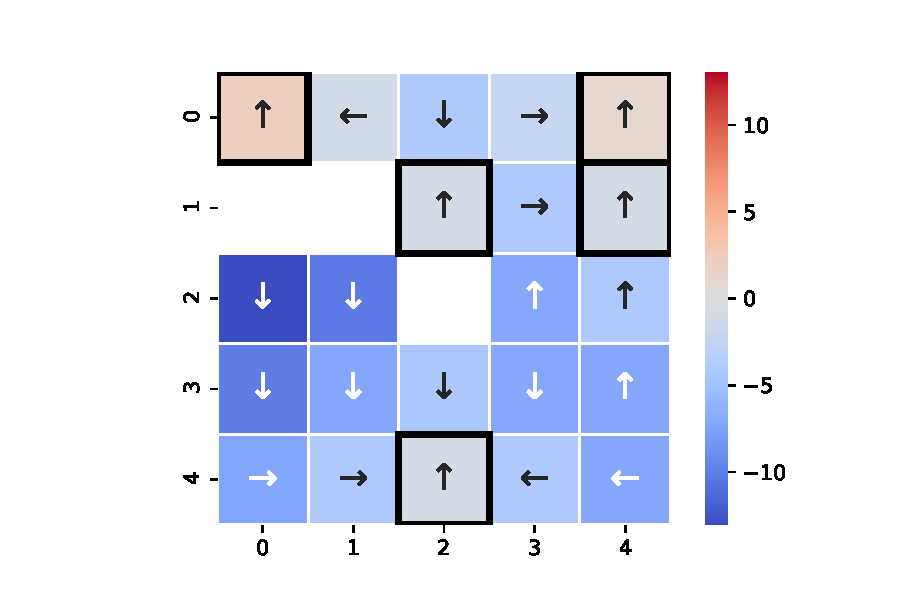
\includegraphics[width=0.5\textwidth, angle=0]{figures/e2_policy_1.pdf}
\end{figure}
\begin{figure}
    \caption{Optimal policy for transition cost 0.46 on board 5x5}
    \label{fig:e2p2}
        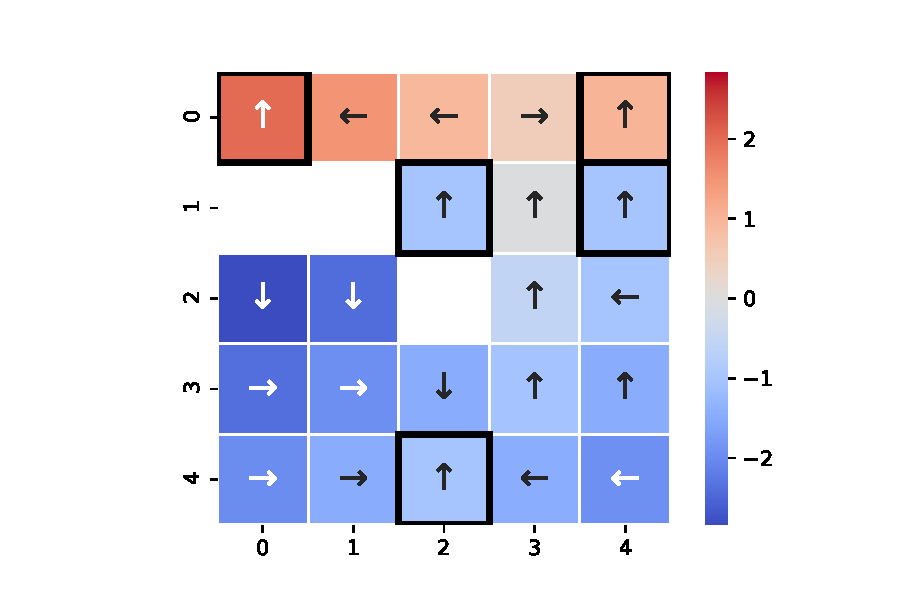
\includegraphics[width=0.5\textwidth, angle=0]{figures/e2_policy_2.pdf}
\end{figure}
\begin{figure}
    \caption{Optimal policy for transition cost 0.27 on board 5x5}
    \label{fig:e2p3}
        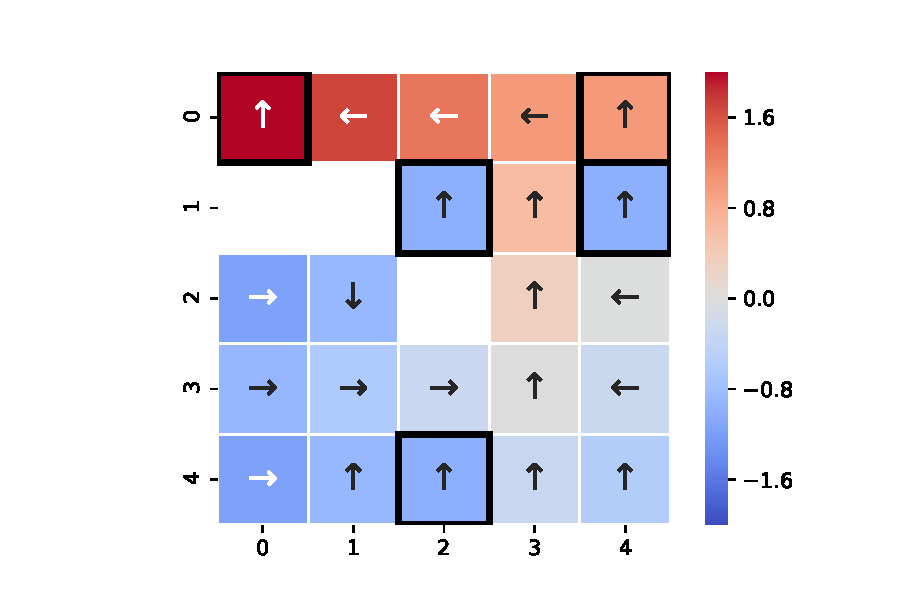
\includegraphics[width=0.5\textwidth, angle=0]{figures/e2_policy_3.pdf}
\end{figure}

I present you with some of the policies here. The optimal policy for transition cost 2.92 can be seen in figure \ref{fig:e2p1}. The policy for 0.46 in figure \ref{fig:e2p2}. And for 0.27 in figure \ref{fig:e2p3}.
The arrows indicate the direction to destination state taken by the policy and the color of each
block is the value of that state.

We can see, that the willingness of taking an action decreases with higher cost. It can be seen in figure \ref{fig:e2p2} and figure \ref{fig:e2p1}, that it is better to
take a -1 action instead of going for higher valued state.



\section*{Experiment 3}\label{sec:experiment3}
In this experiment I have decided to look at the correlation of probability and the transition cost. Specifically how they influence the value of some of the states together.
The result is a heatmap, where the color is given by the value of the state with the probability on the x axis and the transition cost on the y axis. The test was done on 3x4 grid.
Few chosen states are presented in figure \ref{fig:e3_1} for state 10 and in figure \ref{fig:e3_2} for state 11.

\begin{figure}
    \caption{Heatmap showing influence of probability and transition on the transition cost of value of state 10 of board 3x4}
    \label{fig:e3_1}
        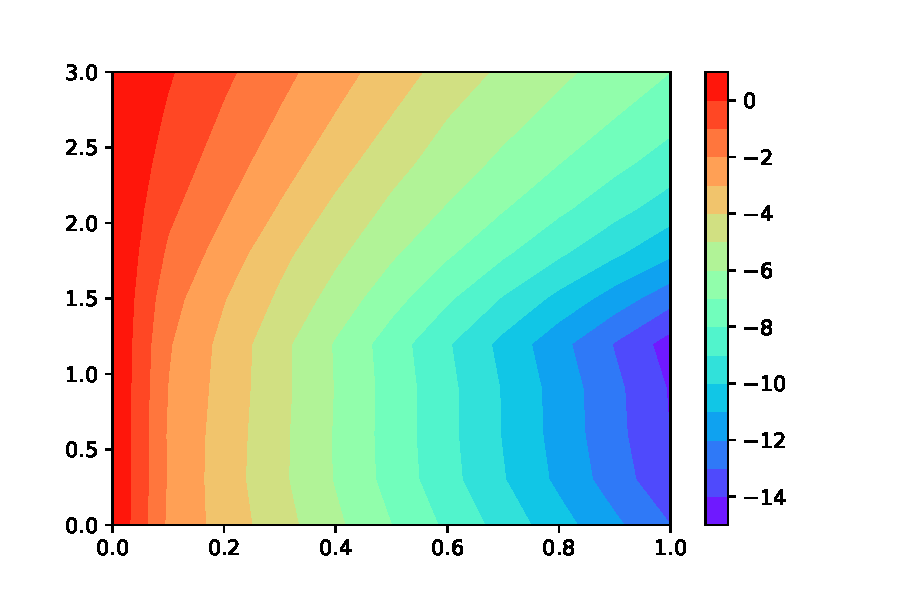
\includegraphics[width=0.5\textwidth, angle=0]{figures/e3_1.pdf}
\end{figure}
\begin{figure}
    \caption{Heatmap showing influence of probability and transition on the transition cost of value of state 11 of board 3x4}
    \label{fig:e3_2}    
        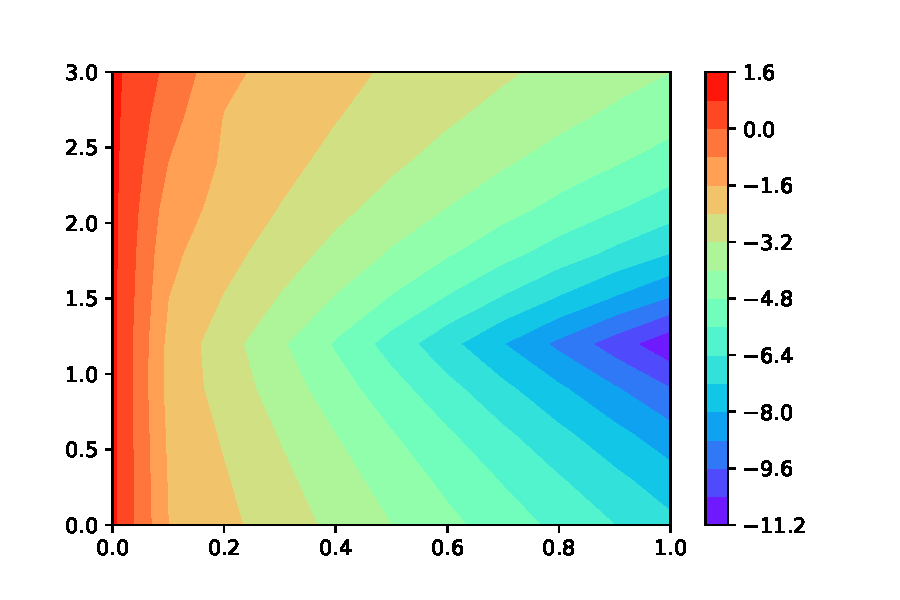
\includegraphics[width=0.5\textwidth, angle=0]{figures/e3_2.pdf}
\end{figure}

In the heatmap, it can be seen, that the willingness of
of taking an action decreases with lower probability and decreases with higher transition cost as expected.

\section*{Experiment 4}\label{sec:experiment4}

\begin{figure}
    \caption{Comparison of speed of convergence of several algorithm for best policy estimation.}
    \label{fig:e4}
        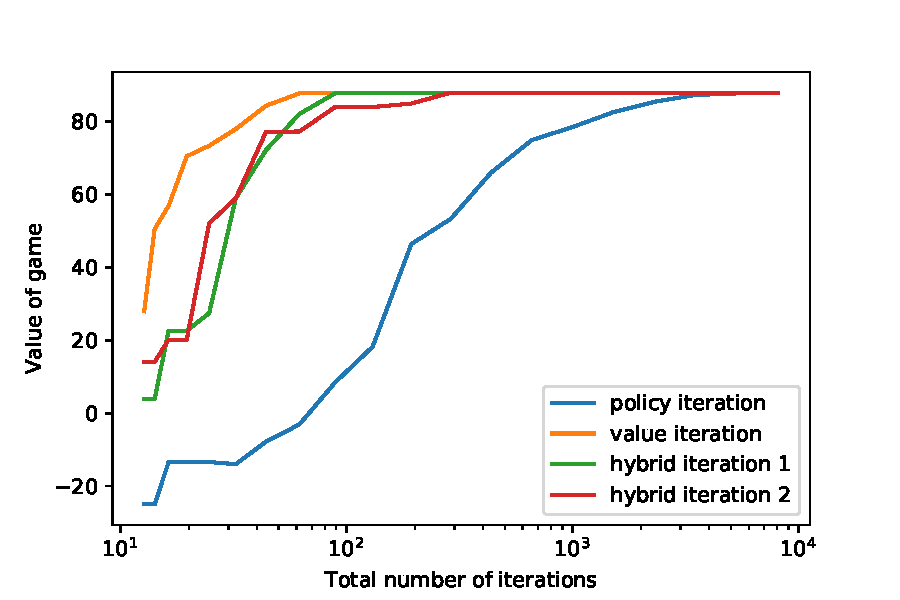
\includegraphics[width=0.5\textwidth, angle=0]{figures/e4.pdf}
\end{figure}

In my final experiment I compared the the value vs. the policy iteration. Furthermore I modified the policy iteration to the "hybrid" iteration and compared it with the policy and the value iterations. 
First I will present you with my modification of the policy iteration which I call "hybrid" iteration.
In the policy iteration, a policy is chosen at the beginning and then the value of the board is calculated for this policy.
The value of the board is calculated in several iterations. Then the optimal policy for that value is chosen and the process repeats.
My modification was to persist the value between iterations and reduce the number of iterations in each policy iteration needed to get the
value of that policy. The objective of this modification is, that at the beginning the
value iteration is too unstable because the policy changes too often. After it gets stable there is no need to make so much iterations for value calculation in
each policy iteration, because the value gets more stable. My approach is somewhere in the middle between value and policy iterations.
First it acts as the policy iteration and with more iterations it becames more like the value iteration.

All approaches are compared in figure \ref{fig:e4}.
The plot has the joint number of iterations on the x axis and total value of the board on the y axis.
For the policy iteration the number of iterations is distributed equally for the inner iterations and policy iterations. Their product
is the same as for value iteration. For the "hybrid" approach, I had chosen two strategies. One of them should act first as the policy iteration and then as the value iteration.
The second algorithm is the same as the policy iteration, but is persists the value of the board between iterations.

The experiment was conducted on 12x6 board. The value estimation appeared to be the best algorithm for this problem,
the "hybrid" approach 1 was second, closely followed by the second "hybrid" approach. The policy iteration was the worst for this scenerio. 

\appendices
\section{Transform function}\label{sec:transform_function}

\begin{figure}
    \caption{The transform function [0, 1) -> [0, $\infty$)}
    \label{fig:e2transform}
        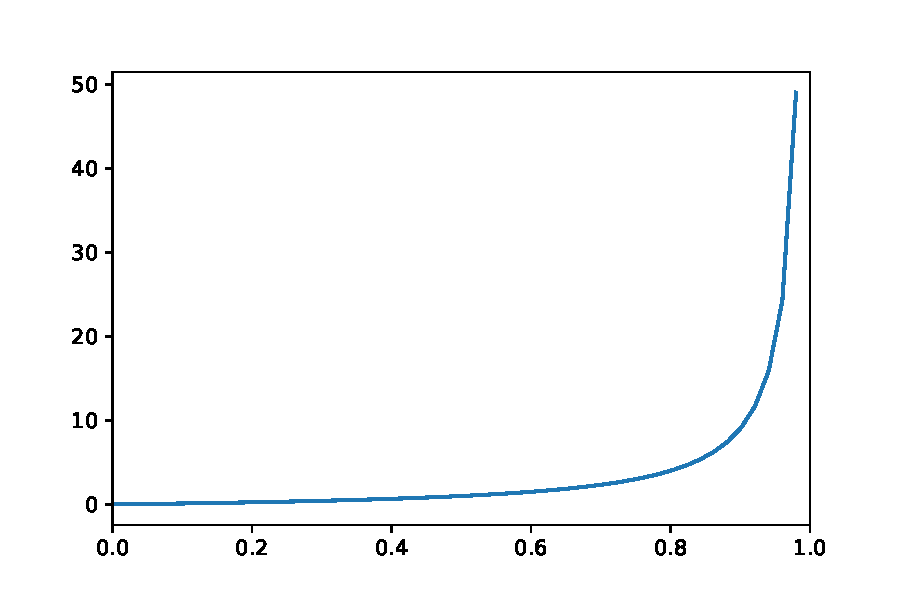
\includegraphics[width=0.5\textwidth, angle=0]{figures/e2_trans.pdf}
\end{figure}

In this section, the transform function used in the second experiment is described.
This function takes values in range [0, 1) and transforms them to the interval [0, $\infty$).
In my experiment, I have chosen this function:
\begin{equation}
    (1 / (1 - X)) - 1
\end{equation}
The plot of this function can be seen in the figure \ref{fig:e2transform}.
\end{document}


